% Created 2024-05-02 Thu 19:47
% Intended LaTeX compiler: pdflatex
\documentclass[conference]{IEEEtran}{}
                      \usepackage{lmodern} % Ensures we have the right font
\usepackage[T1]{fontenc}
\usepackage[utf8]{inputenc}
\usepackage{graphicx}
\usepackage{amsmath, amsthm, amssymb}
\usepackage[table, xcdraw]{xcolor}
\renewcommand{\thesection}{\Roman{section}}
\renewcommand{\thesubsection}{}
\renewcommand{\thesubsubsection}{}
\definecolor{bblue}{HTML}{0645AD}
\usepackage[colorlinks]{hyperref}
\hypersetup{colorlinks, linkcolor=blue, urlcolor=bblue}
\usepackage{titling}
\setlength{\droptitle}{-6em}
\setlength{\parindent}{12pt}
\setlength{\parskip}{0em}
\usepackage[stretch=10]{microtype}
\usepackage{hyphenat}
\usepackage{ragged2e}
\usepackage{subfig} % Subfigures (not needed in Org I think)
\usepackage{hyperref} % Links
\usepackage{listings} % Code highlighting
\usepackage[top=1in, bottom=1.00in, left=0.85in, right=0.85in]{geometry}
\renewcommand{\baselinestretch}{1.00}
\usepackage[explicit]{titlesec}
\pretitle{\begin{center}\fontsize{20pt}{20pt}\selectfont}
\posttitle{\par\end{center}}
\preauthor{\begin{center}\vspace{-6bp}\fontsize{12pt}{12pt}\selectfont}
\postauthor{\par\end{center}\vspace{-25bp}}
\predate{\begin{center}\fontsize{12pt}{12pt}\selectfont\vspace{1em}}
\postdate{\par\end{center}\vspace{0em}}
\titlespacing\section{0pt}{5pt}{5pt} % left margin, space before section header, space after section header
\titlespacing\subsection{0pt}{5pt}{2pt} % left margin, space before subsection header, space after subsection header
\titlespacing\subsubsection{0pt}{5pt}{-2pt} % left margin, space before subsection header, space after subsection header
\usepackage{enumitem}
\setlist{itemsep=-2pt} % or \setlist{noitemsep} to leave space around whole list
\usepackage{listings}
\author{jmowry4@vols.utk.edu}
\date{4/16/24}
\title{\textbf{Maximizing Requests per Second on a Single Thread through \texttt{io\_uring}}\\\medskip
\large Jackson Mowry}
\hypersetup{
 pdfauthor={jmowry4@vols.utk.edu},
 pdftitle={\textbf{Maximizing Requests per Second on a Single Thread through \texttt{io\_uring}}},
 pdfkeywords={},
 pdfsubject={},
 pdfcreator={Emacs 29.3 (Org mode 9.7)}, 
 pdflang={English}}
\usepackage{calc}
\newlength{\cslhangindent}
\setlength{\cslhangindent}{1.5em}
\newlength{\csllabelsep}
\setlength{\csllabelsep}{0.6em}
\newlength{\csllabelwidth}
\setlength{\csllabelwidth}{0.45em * 4}
\newenvironment{cslbibliography}[2] % 1st arg. is hanging-indent, 2nd entry spacing.
 {% By default, paragraphs are not indented.
  \setlength{\parindent}{0pt}
  % Hanging indent is turned on when first argument is 1.
  \ifodd #1
  \let\oldpar\par
  \def\par{\hangindent=\cslhangindent\oldpar}
  \fi
  % Set entry spacing based on the second argument.
  \setlength{\parskip}{\parskip +  #2\baselineskip}
 }%
 {}
\newcommand{\cslblock}[1]{#1\hfill\break}
\newcommand{\cslleftmargin}[1]{\parbox[t]{\csllabelsep + \csllabelwidth}{#1}}
\newcommand{\cslrightinline}[1]
  {\parbox[t]{\linewidth - \csllabelsep - \csllabelwidth}{#1}\break}
\newcommand{\cslindent}[1]{\hspace{\cslhangindent}#1}
\newcommand{\cslbibitem}[2]
  {\leavevmode\vadjust pre{\hypertarget{citeproc_bib_item_#1}{}}#2}
\makeatletter
\newcommand{\cslcitation}[2]
 {\protect\hyper@linkstart{cite}{citeproc_bib_item_#1}#2\hyper@linkend}
\makeatother\begin{document}

\maketitle
\begin{abstract}
This research paper investigates the transformative potential of \texttt{io\_uring} in scaling HTTP web servers to accommodate the needs of numerous concurrent clients. Despite the extensive exploration of various scaling techniques, little attention has been paid to the potential paradigm shift that \texttt{io\_uring} may introduce in asynchronous I/O architectures. \texttt{io\_uring} enables the handling of workloads traditionally confined to highly parallelized systems. This paper aims to explore the implications of \texttt{io\_uring} on asynchronous I/O systems, shedding light on its promise for enhancing server scalability and performance in the face of ever increasing demands.
\end{abstract}
\section{Introduction}
\label{sec:org2c7fc68}
Web servers are a class of software that sit between nearly every interaction a client makes on their device, and access to the files hosted on a server. Despite this fact their implementations mainly use software designs of the past, due to the fact that for most use cases they are ``good enough''. It is true that even a naive HTTP server can serve thousands of requests per second \cslcitation{1}{[1]}, \cslcitation{2}{[2]}, which easily surpasses the needs of most users. However, when it comes time to handle a higher load the same architecture has only two ways to scale. The server can either be rewritten to take advantage of multiple CPU cores, or it can have multiple instances running behind a load balancer \cslcitation{3}{[3]}.

The root of this issue lies in the fact that these workloads are still inhrently synchronous at some level  (excluding \texttt{aio} based solutions, which are rare \cslcitation{4}{[4]}), which leads to large requests slowing the time needed to complete each request. \texttt{io\_uring} presents a true asynchronous io system with its introduction into the Linux kernel (version 5.1) \cslcitation{4}{[4]}, \cslcitation{5}{[5]}. An exciting new space for high performance single core servers now exists, in this paper we will see how \texttt{io\_uring} can fill that gap. To date \texttt{io\_uring} has not been implemented in mainstream web server applications, this paper serves to illuminate the potential benefits, to both speed and latency, of the latest in asynchronous io technology.
\section{Previous Work}
\label{sec:orgf6ca7d6}
Maximizing throughput on asynchronous or multiplexed architectures has often focused on \texttt{epoll} as the main differentiating factor\cslcitation{2}{[2]}, \cslcitation{3}{[3]}. The performance of \texttt{epoll} is better than that of synchronous mechanisms like \texttt{select} or \texttt{poll}, but \texttt{epoll} alone is not enough to meet modern demands \cslcitation{6}{[6]}. Instead, web servers often implement complex thread pools to handle massively concurrent workloads \cslcitation{7}{[7]}. By spreading the load out to multiple physical cores, the disadvantages of blocking system calls can be mitigated from a request latency prespective \cslcitation{3}{[3]}.

\texttt{io\_uring} has begun to recieve attention in the storage performance world, where the new architecture allows for high performace systems across all types of file descriptors. This interface allows for performance critical application to both improve performance, and simplify the event handling code, while keeping the important logic entirely in user-space \cslcitation{8}{[8]}, \cslcitation{9}{[9]}, \cslcitation{10}{[10]}.

The increasing momentum around \texttt{io\_uring} has drawn more eyes to the system, leading to more features being added \cslcitation{11}{[11]}, and vulnerabilities being patched \cslcitation{12}{[12]}, \cslcitation{13}{[13]}.
\section{Asynchronous IO}
\label{sec:org2c6d023}
Most if not all system calls used in day to day software are considered ``blocking'', meaning they will only return once the entire function has finished executing. This model allows for programmers to not have to worry about order of execution, as they know their program will run top to bottom without skipping a step. This paradigm was formed under the (correct) assumption that IO was always the bottleneck of an application, however, modern systems are now at the point where CPU is once again becoming a limiting factor \cslcitation{14}{[14]}, \cslcitation{15}{[15]}. To avoid the performance impact of synchronous IO, programmers may choose to design their software around asynchronous IO.

For most applications it may not make sense to perform all system calls concurrently/asyncronously \cslcitation{7}{[7]}. We certainly want slower system calls to complete in the background, but the added overhead of an asynchronous system call may make faster calls worse. We expect to see greater differences in throughput for large files as serving large files synchronously requires the entire file to be sent before moving on to the next connection.
\section{Latency}
\label{sec:org78c5d75}
A common mark of server performance is requests per second \cslcitation{1}{[1]}, \cslcitation{2}{[2]}, but this metric only applies to some workloads. If the goal is to serve many concurrent connections without massive latency, special care needs to be taken to how requests handling is scheduled. Specifically for a file server, the application needs to ensure that requests are being processed concurrently, so that each request has a chance to progress towards completion \cslcitation{16}{[16]}.

\begin{figure*}
\centering
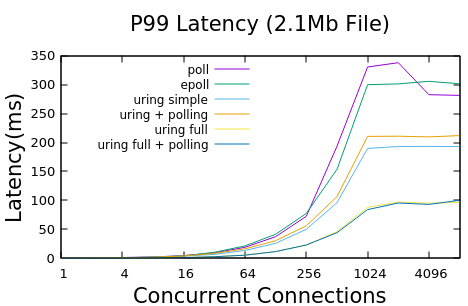
\includegraphics[width=4.5in]{big_latency.png}
\caption{Latency for serving a large file, the full \texttt{io\_uring} server exhibits the best latency curve, half that of simple \texttt{io\_uring}, and a third of either \texttt{poll} or \texttt{epoll}}
\end{figure*}

This problems was first described as the ``C10K'' problem, which references the challenege of handling 10,000 concurrent requests on a server with hardware from 1999. The discussions at the time covered different server architectures, ranging from fully synchronous, to the state of the art, which at the time was the emerging \texttt{aio} system. A general conclusion is that the scalability of web servers is largely dependent on how request handling could be performed concurrently through efficient scheduling \cslcitation{3}{[3]}.

Both \texttt{poll} and \texttt{epoll} (along with other synchronous approaches) fall short in this regard. Due to the linear scanning of all incoming requests, latency will grow quickly as the number of clients increases (Figure 1). A server spread across multiple cores will easily outperform a single core are lower connected clients, but will quickly begin to climb in latency as the number of clients grows. The overhead from spawning a thread per request is not feasible past a certain point. \texttt{io\_uring} is able to avoid this problem by scheduling requests within the kernel, which allows the application to handle an event as soon as it completes \cslcitation{4}{[4]}.
\section{\texttt{aio}}
\label{sec:orgdc919ae}
The \texttt{aio} system in Linux has two implementations, POSIX compliant, and the Linux implementation. Both systems suffer from the same core issue, they are intended to work with regular files, and as such don't play well with sockets. glibc creates a thread pool to perform regular synchronous io off the main thread, giving the illusion of asynchronosity to the user-space program \cslcitation{17}{[17]}.

\texttt{aio} is also very limited in scope, only offering real support for read and write calls \cslcitation{4}{[4]}. This means that without splicing together features from different asynchronous IO frameworks an application will still have to rely heavily on blocking system calls \cslcitation{11}{[11]}.

For all of these reasons \texttt{aio} is generally avoided in application code.
\section{\texttt{epoll}}
\label{sec:org49bb87d}
\texttt{epoll} is kernel based implementation of \texttt{poll}, with both providing a way to monitor a range of file descriptors, and alerting the user when one or many are ready for IO. It has become a common architecture for web servers and other asychronous io systems to be built on top of. Most notably to implement the primatives golang's \texttt{net/http} package is built upon, and \texttt{libuv} which powers the Node.js event loop.

\texttt{epoll} expands on the original ideas of \texttt{poll} by sharing a list of file descriptors between the user and kernel, allowing for a more efficient loop once events are ready. When any number of file descriptors are ready for IO they will be placed in a separate shared list, which the user can then perform the desired action on \cslcitation{18}{[18]}.

This architecture allows for a single thread to handle a large of active file descriptors, only slowing down to perform the synchronous operations like reading or writing \cslcitation{19}{[19]}. The actual implementation does not directly allow for asynchronous sending or recieving of data, instead relying on non-blocking file descriptors, which can be polled for completion \cslcitation{18}{[18]}. One downside of \texttt{epoll} is that it does not behave consistently across file descriptors of different types.

While it is true that recieving data from a socket can block, which \texttt{epoll} is aware of, regular files do not exhibit the same behavior.Due to \texttt{epoll}'s handling of regular files they will always be placed on the ready list immedietly. On Linux read and write calls to a file should not block, but as we all know this is not true. You can make a write call and expect it to complete instantly, but if the kernels write cache is full, you will have to wait. The same goes for a read call which can blocked if the file is on a slow drive \cslcitation{6}{[6]}.
\section{\texttt{io\_uring}}
\label{sec:org809730d}
\texttt{io\_uring} is the latest attempt at adding asynchronous operations to Linux. The design intentions show that many lessons have been  learned from shortcomings of previous asynchronous IO systems on Linux. Not only does \texttt{io\_uring} provide a common interface across all types of file descriptors, it also implements most IO systems calls in an asyncronous fashion \cslcitation{4}{[4]}, \cslcitation{5}{[5]}, \cslcitation{11}{[11]}.

\begin{figure*}
\centering
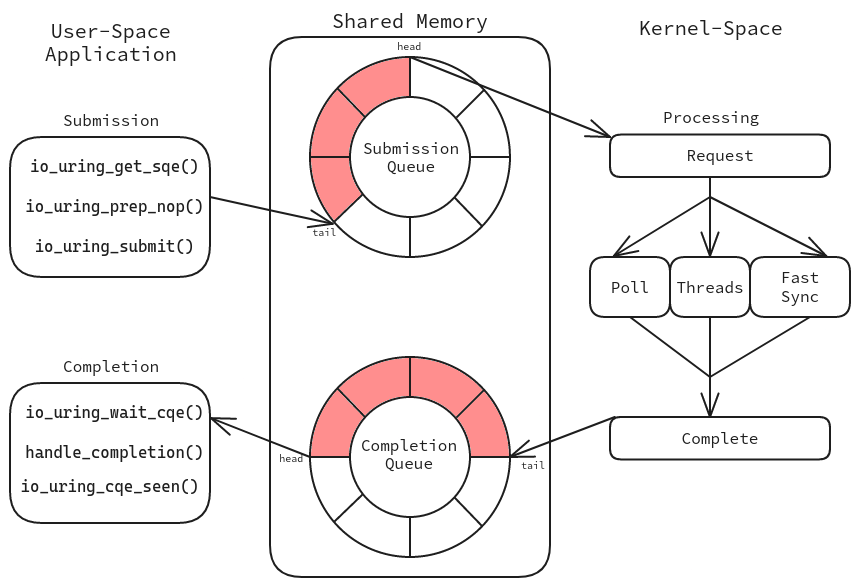
\includegraphics[width=.9\linewidth]{uring_diagram.png}
\caption{\texttt{io\_uring} by sharing a submission and completion ring buffer between the user and kernel. This allows efficient job submission/completion without the use of system calls.}
\end{figure*}

The design can be broken down into two distinct parts, a job submission queue, and a job completion queue, both implemented via ring buffers shared between the kernel and user space (Figure 2). At a basic level each submission is a combination of an op code defining which system call to perform, and the associated arguments \cslcitation{4}{[4]}. If the user desires to keep track of a job they can associate user data with a submission, which takes the form of an 64-bit integer, commonly used to hold a pointer to an object whoes lifetime is tied to the job completion.

Once a job is complete it is placed in the completion queue, which an application can pull from. Completions come in the form of a result code, and the associated user data. The result code is analogous to the return value from regular blocking system calls with one exception, Due to the concurrent execution of submissions the system cannot garuntee that the \texttt{ERRNO} associated with each system call will still be properly set when a user recieves a completion. Instead, \texttt{ERRNO} is placed in the completion struct, with its value negated so that it will not be confused with a successful execution \cslcitation{6}{[6]}.

\texttt{io\_uring} also offers another distinct advantage over the other asynchronous io methods presented here. Jobs can be submitted through a system call, or by having the kernel continuously poll the submission queue using a separate thread. This allows for a program to operate entirely in user space, avoiding system calls which have become even more costly in the age of speculative execution mitigations (Table 1)\cslcitation{11}{[11]}.

In systems where response time is the highest concern, submission queue polling will likely be the best choice due to eliminating a system call per request. However, if a system is not expecting high numbers of concurrent connections, it would be best to stick with submissions as system calls. If a space bursty workload would still benefit from submission queue polling the kernel thread can be told to sleep after a certain interval, specified by \texttt{sq\_thread\_idle}. We will explore both methods of job submission to see where their advantages lie.

Being the latest in the asyncronous IO space \texttt{io\_uring} is still lacking some features. Most notably is missing system calls, and event notification on a submission/completion level. Most missing system calls can be implemented without changing the underlying system \cslcitation{6}{[6]}, \cslcitation{11}{[11]}.
\section{System Calls}
\label{sec:orge419ce6}
One of the major mitigations put into place after the speculative execution attacks were discovered (spectre and meltdown) was isolation of kernel and user space memory. This slows system calls as they must switch to privlaged execution and the kernel address space to perform the operation, and switch back once they're done, requiring a TLB flush before returning to user mode \cslcitation{14}{[14]}, \cslcitation{15}{[15]}, \cslcitation{20}{[20]}, \cslcitation{21}{[21]}, \cslcitation{22}{[22]}.

To mitigate this, modern software systems have transitioned to a model where system calls are avoided, sometimes entirely \cslcitation{23}{[23]}. The most obvious implementations of this are systems that manage memory allocations themselves, or those that manage files using shared memory \cslcitation{24}{[24]}.

\texttt{io\_uring} allows the program to avoid system calls for job submission, meaning that an application can work entirely in userspace, without the need for costly system calls. This reduces the number of system calls from at a minimum 4 (accept, read, write, close) in a synchronous server, to a potential 0\footnote{Once \texttt{sendfile} is implemented this will be possible, for now one call to \texttt{pipe}, and two calls to \texttt{fcntl} are required to mimic the behavior.\label{orgdc10cfb}} in an \texttt{io\_uring} based approach.

\begin{table}[htbp]
\caption{System calls needed to process a request on each server architecture}
\centering
\begin{tabular}{|l|c|}
Server Architecture & System Calls per Request\\
\hline
poll & 10\\
epoll & 8\\
io\textsubscript{\_}uring simple & 7\\
io\textsubscript{\_}uring simple + polling & 6\\
io\textsubscript{\_}uring full & 7\\
io\textsubscript{\_}uring full + polling & 3\textsuperscript{\ref{orgdc10cfb}}\\
\end{tabular}
\end{table}

Another advantage of \texttt{io\_uring} comes in its ability to schedule many jobs concurrently, with IO heavy requests being handled off the main thread. By processing all IO in the background, clients requesting large files do not block others looking for small files. This is a major advantage over synchronous servers where either an entire program is blocking reading/writing a file, or a thread is held up waiting. This can slow the overall throughput of these systems, whereas an asynchronous implementation would proceed handling other clients while a file is being read.

Web servers may try to combat the cost of system calls by using auxiliary threads to handle either entire requests, or smaller portions. This approach works until a certain point, as the overthread of spawning an operating system thread is non-trivial. The best approach will likely vary application to application, as certain applications may require heavy synchronous computations, which a single thread would not be able to handle \cslcitation{7}{[7]}.
\section{Methods \& Implementation}
\label{sec:org10c8b56}
Testing will include an \texttt{epoll} server, four distinct \texttt{io\_uring} servers, and a sixth synchronous server using \texttt{poll}. Servers will parse a request, open a file, respond with the appropriate headers, send the file, and finally close the connection. Performance testing using \texttt{wrk} at \{1, 4, 8, 16, 32, 64, 128, 256, 512, 1024, 2048, 4096, 8192\} concurrent connections run over 30 seconds, with the mean of 3 runs reported for each metric. Servers will also be tested across a range of file sizes \{9B, 12KB, 2.1Mb\}.

Each server will folow a similar pattern to minimize differences between implementations. After parsing the request to determine which file is being request, the file will then be opened. In order to send back valid HTTP headers, \texttt{stat} is called on the file to gather the file size. The response headers can then be formed and sent back using \texttt{send}. The final step is to send back the file contents using \texttt{sendfile}, which we will emulate using \texttt{splice} in \textbf{uring full}.

The first general purpose web server, named \textbf{uring simple}, will perform only the \texttt{accept}, \texttt{read}, and \texttt{close} system calls via asynchronous mechanisms, with the rest of the work handled synchronously. The application follows a simple state machine where a connection is either in \texttt{ACCEPT}, \texttt{READ}, or \texttt{WRITE/CLOSE}.

\textbf{uring full} will replace every system call (except for \texttt{pipe} which does not yet exist) with their asynchronous versions. The state machine follows a similar pattern adding \texttt{CLOSE\_FILE}, \texttt{CLOSE\_SOCKET}, \texttt{CLOSE\_PIPE}, \texttt{OPEN}, \texttt{SPLICE}, \texttt{STATX}, and \texttt{SEND}.

Both \texttt{io\_uring} servers will have submission queue polling enabled (\textbf{uring simple + SQP}) (\textbf{uring full + SQP}) as additional observation points.
\section{Results}
\label{sec:orgdf9533f}
\subsection{Latency}
\label{sec:org8f361cd}
As expected, the synchronous \texttt{poll} based server experiences substantial growth in latency as the number of concurrent requests in increased. This is due to the fact the scanning the list of watched file descriptors happens in linear time as each is checked for a \texttt{POLLIN} event. The \texttt{epoll} server is able to maintain a similar latency to either \texttt{io\_uring} server until 128 concurrent requests when it begins to climb rapidly. Latency continues to grow with connections, and would be expected to continue rising.

Both \texttt{io\_uring} servers exhibit similar P99 latency, quickly reaching a plateau around 25ms from 1024 concurrent requests and beyond (Figure 4). Submission queue polling increases latency by a fixed amount across the entire test range, with the change having the largest impact when serving small files, as was predicted. For the \textbf{uring simple} and \textbf{uring full} servers, enabling polling dropped latency by 67\% and 53\% respectivly (Figure 3).

\begin{center}
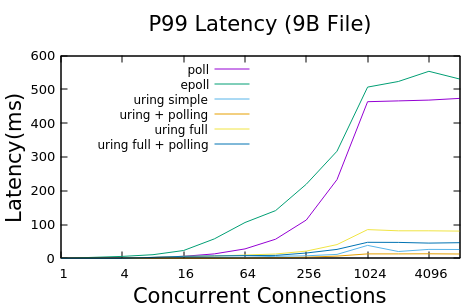
\includegraphics[width=3.35in]{small_latency.png}
\captionof{figure}{Both full and simple \texttt{io\_uring} servers show similar latency characteristics with small files, whereas either synchronous option is up to 10x slower}
\end{center}

While serving small files still benefits substantially from \texttt{io\_uring}, the simple \texttt{io\_uring} server beats a full server by a factor of 2x (Figure 3). A small file tends to be less performance bound by disk IO, as the entire file can easily be read and written in a single page. Moving up to a medium sized file (12Kb) we see that the gap between either \texttt{io\_uring} remains about the same, just around 2x (Figure 4). It is not until the large file is requested that a full \texttt{io\_uring} server begins to show its advantages. At a full 8192 connection load the simple \texttt{io\_uring} server peaks at 200ms of latency, whereas the full \texttt{io\_uring} server just begins to push 100ms. Either synchronous server continues to climb in latency up until a peak of 300ms at full load (Figure 1).

\begin{center}
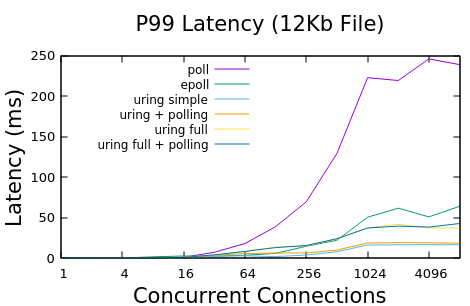
\includegraphics[width=3.35in]{./med_latency.png}
\captionof{figure}{With medium sized files simple \texttt{io\_uring} performs the best at about half the latency of the full \texttt{io\_uring} server. \texttt{poll} begins to show major disadvantages compare to any other option.}
\end{center}
\subsection{Throughput}
\label{sec:orgd450696}
Throughput of the synchronous server follows our expectations, a nearly flat line across the entire testing range (Figure 5). The rate at which we can push data over the wire is entirely limited by the fact that each request is handled one at a time, which is dependent on the time in which we are blocked in system calls. For simple applications this approach may be enough to handle the workload, and it comes with the upside that a \texttt{poll} implementation is a much simpler architecture.

\begin{center}
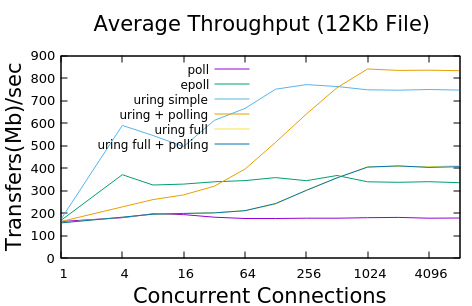
\includegraphics[width=3.35in]{med_throughput.png}
\captionof{figure}{Both synchronous servers exhibit a very similar throughput across the entire request range. Either \texttt{io\_uring} server with submission queue polling performs worse at lower concurrent requests, which hits a crossover point and ultamitely exceeds the simple \texttt{io\_uring} server at 512 connected clients.}
\end{center}

\texttt{epoll} exhibits nearly the same behavior as the poll based implementation, only at a higher overall throughput. We see no degradation in throughput for either server up to 8192 concurrent requests. The advantage for \texttt{epoll} comes in the fact that it's ``work queue'' is only populated with requests that have data ready, meaning that each file descriptor can have work done without having to check its status.

\textbf{uring simple} without submission queue polling quickly reaches its maximum throughput at 128 concurrent requests, which the server is able to maintain all the way up through 8192 concurrent requests (Figure 5). This equates to a maximum throughput of around 750MB/s, or \textasciitilde{}6Gbit/s, serving a 12KB text file to each client. When submission queue polling is enabled we see an interesting shift in throughput. A much lower throughput is seen at lower concurrent requests, which quickly jumps past the original implementation at 512 concurrent requests. From 512 requests and beyond, a gap of just under 10,000 requests per second is maintained. This equates to a gap of around 100MB/s, or 0.8Gbit/s.

As suspected the \textbf{uring full} server is still slower for medium sized files. Peaking at just over 400Mb/s with or without submission queue polling while serving a 12Kb file, a value under half that achieved by \textbf{uring simple}. The performance scales in a same manner as \textbf{uring simple}, at about half the overall throughput (Figure 5). We observe no performance impacts from enabling submission queue polling.

\begin{figure*}
\centering
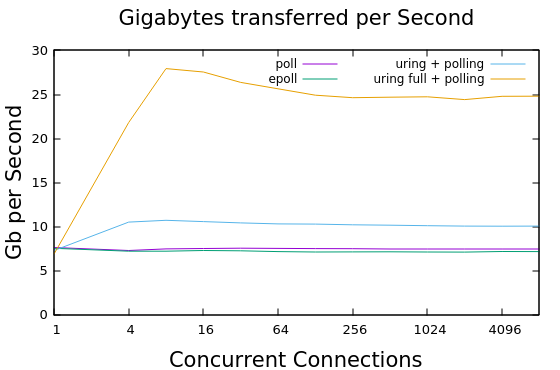
\includegraphics[width=4.5in]{gbps.png}
\caption{Both synchronous servers, and the simple \texttt{io\_uring} server show near similar performace across the entire request range, whereas the full \texttt{io\_uring} server beats the servers by 3.5x and 2.5x respectively.}
\end{figure*}

Testing with large file sizes begins to highlight the advantages from the newer \texttt{io\_uring} system. When clients request a 2.1Mb file we finally begin to see that \textbf{uring full} has major advantages over another other implementation. Without blocking each request on a single synchronous path we greatly increase throughput, and decrease latency. Both synchronous servers, and the simple \texttt{io\_uring} server spend the majority of their runtime blocked in system calls, meaning that even though we have thousands of connected clients, we cannot concurrently send any information to multiple clients.

The largest contributing factor to decreased throughput (and thus increased latency) is the sending of the large 2.1Mb file, which is entirely mitigated when using asynchronous IO. This results in \textbf{uring full} beating \texttt{epoll} by 3.5x, and a \textbf{uring simple} by 2.5x. At 8 concurrent clients \textbf{uring full} achieves a peak throughput of 27.94GB/s, settling in to just around 24.8GB/s for the remaining tests (Figure 6).

\begin{center}
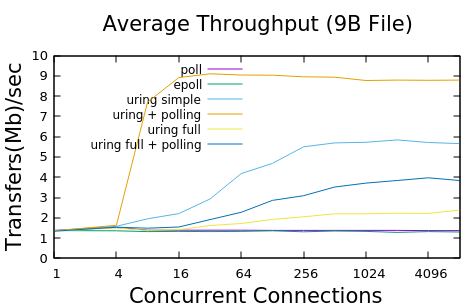
\includegraphics[width=3.35in]{small_throughput.png}
\captionof{figure}{Asynchronous task completion overhead dominates throughput with smaller files, leading to \textbf{uring simple} performing better then \textbf{uring full}}
\end{center}

We see the opposite results when testing a smaller 9 byte file, as the overhead of processing system calls asynchronously greatly decreases overall throughput. The best performer with small files was \textbf{uring simple} with submission queue polling enabled, which managed 8.79MB/s at 8192 concurrent connections. \textbf{uring full} was able to achieve just under half the throughput (3.84MB/s), still beating either synchronous server (\textasciitilde{}1.30MB/s) (Figure 7).
\section{Discussion}
\label{sec:orga842677}
Either asynchronous implementation offers obvious advantages over an entirely synchronous server. As discussed before, one potential disadvantage with \texttt{epoll} is that it only works well with sockets, or files opened in an unbuffered/direct mode. If an application needs to do more than accept an incoming connection on a socket and send back a response, \texttt{epoll} will not be useful for other operations. \texttt{io\_uring} on the other hand offers a uniform interface for the entire range of IO operations. This consistent handling of different file descriptors allows for the programmer to simplify their application to a more robust state machine.

A fully asynchronous server is able to scale in both throughput and latency, which is desireable for many applications. This increase in performance also comes with the simplicity of running on a single user space thread. A single threaded application generally limits the need for concurrency control mechanisms, which can slow the execution of a program.

\texttt{io\_uring} has shown that with its superior implementation it can out perform the contemporary way we build single-threaded web servers. Showing a 75.95\% improvement (85.01\% with SQ polling enabled) in throughput over the \texttt{epoll} based server at 8192 concurrent requests when serving a 12Kb file. The worst case latency of an \texttt{io\_uring} server also scales better than \texttt{epoll}, exhibiting 1/4 the latency at 8192 concurrent requests (Figure 4).

The general performance gap only grows as the response size does as well. When serving a 9 byte file \texttt{io\_uring} exhibits a 2x increase in throughput, which grows to over 2.5x at 12Kb, and finally 3.5x for a 2.1Mb file. This follows the long known trend that asynchronous operations help IO bound applications scale. As file size increases we would expect to see the same trend of decreased latency and increase throughput.
\section{Future Work}
\label{sec:orgf78cd47}
More work is needed to explore the different performance impacts of various asynchronous calls through \texttt{io\_uring}. Theoretically, a server performing very few systems calls should outperform one doing many system calls, but as we have observed, this is not always the case. Once a few more of the key systems calls have been implemented (pipe, and sendfile specifically) performance testing should once again be performed.

In order to mitigate the impacts of submission queue polling, an hybrid architecture that can dynamically toggle polling on an off should be explored. This could be implemented either with a load balancer which can switch to a different server when overload load reaches some threshold, or within the server by using two separate \texttt{io\_uring} instances. This behavior is likely achievable due to the tunable spindown time of the polling thread, which can essentially be disabled by setting this value appropriately.
\section{References}
\label{sec:org98b0dc8}
\begin{cslbibliography}{1}{0}
\cslbibitem{1}{\cslleftmargin{[1]}\cslrightinline{G. Banga and P. Druschel, “Measuring the capacity of a web server,” in \textit{Usenix symposium on internet technologies and systems (usits 97)}, 1997.}}

\cslbibitem{2}{\cslleftmargin{[2]}\cslrightinline{D. Pariag, T. Brecht, A. Harji, P. Buhr, A. Shukla, and D. R. Cheriton, “Comparing the performance of web server architectures,” \textit{Acm sigops operating systems review}, vol. 41, no. 3, pp. 231–243, 2007.}}

\cslbibitem{3}{\cslleftmargin{[3]}\cslrightinline{D. Kegel, “The c10k problem,” \textit{Http://www. kegel. com/c10k. html}, 2006.}}

\cslbibitem{4}{\cslleftmargin{[4]}\cslrightinline{J. Axboe, “Efficient io with io\_uring,” \textit{Kernel.dk}. Available: \url{https://kernel.dk/io_uring.pdf}}}

\cslbibitem{5}{\cslleftmargin{[5]}\cslrightinline{J. Corbet, “Ringing in a new asynchronous i/o api,” \textit{Lwn.net}. Available: \url{https://lwn.net/Articles/776703/}}}

\cslbibitem{6}{\cslleftmargin{[6]}\cslrightinline{S. Hussain, “Welcome to lord of the io\_uring,” \textit{Welcome to lord of the io\_uring - lord of the io\_uring documentation}. Available: \url{https://unixism.net/loti/}}}

\cslbibitem{7}{\cslleftmargin{[7]}\cslrightinline{J. Ousterhout, “Why threads are a bad idea (for most purposes).” Talk, Sep. 1995.}}

\cslbibitem{8}{\cslleftmargin{[8]}\cslrightinline{D. Didona, J. Pfefferle, N. Ioannou, B. Metzler, and A. Trivedi, “Understanding modern storage apis: a systematic study of libaio, spdk, and io\_uring,” in \textit{Proceedings of the 15th acm international conference on systems and storage}, 2022, pp. 120–127.}}

\cslbibitem{9}{\cslleftmargin{[9]}\cslrightinline{Z. Ren and A. Trivedi, “Performance characterization of modern storage stacks: Posix i/o, libaio, spdk, and io\_uring,” in \textit{Proceedings of the 3rd workshop on challenges and opportunities of efficient and performant storage systems}, 2023, pp. 35–45.}}

\cslbibitem{10}{\cslleftmargin{[10]}\cslrightinline{T. Endo and S. M. S. Al-Mashni, “Comparative evaluation of asynchronous io interface between io\_uring and libaio implemented in a nosql db for ssds,” \textit{情報処理学会第 82 回全国大会}, vol. 5, p. 02, 2020.}}

\cslbibitem{11}{\cslleftmargin{[11]}\cslrightinline{J. Axboe, “What’s new with io\\_uring,” \textit{Kernel recipes}, 2022.}}

\cslbibitem{12}{\cslleftmargin{[12]}\cslrightinline{W. He, H. Lu, F. Zhang, and S. Wang, “Ringguard: Guard io\_uring with ebpf,” in \textit{Proceedings of the 1st workshop on ebpf and kernel extensions}, 2023, pp. 56–62.}}

\cslbibitem{13}{\cslleftmargin{[13]}\cslrightinline{J. Xu \textit{et al.}, “Mock: Optimizing kernel fuzzing mutation with context-aware dependency.”}}

\cslbibitem{14}{\cslleftmargin{[14]}\cslrightinline{P. Enberg, A. Rao, and S. Tarkoma, “I/o is faster than the cpu: Let’s partition resources and eliminate (most) os abstractions,” in \textit{Proceedings of the workshop on hot topics in operating systems}, 2019, pp. 81–87.}}

\cslbibitem{15}{\cslleftmargin{[15]}\cslrightinline{Y. Zhong \textit{et al.}, “Bpf for storage: an exokernel-inspired approach,” in \textit{Proceedings of the workshop on hot topics in operating systems}, 2021, pp. 128–135.}}

\cslbibitem{16}{\cslleftmargin{[16]}\cslrightinline{S. M. Rumble, D. Ongaro, R. Stutsman, M. Rosenblum, and J. K. Ousterhout, “It’s time for low latency,” in \textit{13th workshop on hot topics in operating systems (hotos xiii)}, 2011.}}

\cslbibitem{17}{\cslleftmargin{[17]}\cslrightinline{S. Bhattacharya, S. Pratt, B. Pulavarty, and J. Morgan, “Asynchronous i/o support in linux 2.5,” in \textit{Proceedings of the linux symposium}, Citeseer, 2003, pp. 371–386.}}

\cslbibitem{18}{\cslleftmargin{[18]}\cslrightinline{L. Gammo, T. Brecht, A. Shukla, and D. Pariag, “Comparing and evaluating epoll, select, and poll event mechanisms,” \textit{Proceedings of the 6th annual ottawa linux symposium}, 2004.}}

\cslbibitem{19}{\cslleftmargin{[19]}\cslrightinline{F. Schmaus, F. Fischer, T. Hönig, and W. Schröder-Preikschat, “Modern concurrency platforms require modern system-call techniques,” \textit{Technical reports / department informatik}, vol. CS-2021, no. 2, 2021.}}

\cslbibitem{20}{\cslleftmargin{[20]}\cslrightinline{M. Löw, “Overview of meltdown and spectre patches and their impacts,” \textit{Advanced microkernel operating systems}, p. 53, 2018.}}

\cslbibitem{21}{\cslleftmargin{[21]}\cslrightinline{A. Prout \textit{et al.}, “Measuring the impact of spectre and meltdown,” in \textit{2018 ieee high performance extreme computing conference (hpec)}, IEEE, 2018, pp. 1–5.}}

\cslbibitem{22}{\cslleftmargin{[22]}\cslrightinline{X. Ren, K. Rodrigues, L. Chen, C. Vega, M. Stumm, and D. Yuan, “An analysis of performance evolution of linux’s core operations,” in \textit{Proceedings of the 27th acm symposium on operating systems principles}, 2019, pp. 554–569.}}

\cslbibitem{23}{\cslleftmargin{[23]}\cslrightinline{L. Gerhorst, B. Herzog, S. Reif, W. Schröder-Preikschat, and T. Hönig, “Anycall: Fast and flexible system-call aggregation,” in \textit{Proceedings of the 11th workshop on programming languages and operating systems}, 2021, pp. 1–8.}}

\cslbibitem{24}{\cslleftmargin{[24]}\cslrightinline{I. TigerBeetle, “Tigerbeetle,” \textit{Tigerbeetle.com}. Available: \url{https://tigerbeetle.com/}}}

\end{cslbibliography}
\end{document}
